\section{Formal Methods}\label{sec:decproc}
Formal methods are a kind of system design techniques which use meticulous mathematical models for the specification, development and verification of software and hardware systems. The application of these kind of methods to the design of both software and hardware systems is supported by the increased reliability and robustness of the resulting systems. In this thesis we are more interested in the use of formal methods as verification techniques: we will consider a finished system and we will try to use the verification techniques in order to enhance its reliability.
In particular the system we will consider is a machine learned controller, therefore in this section we present two of the most popular formal verification techniques used in the verification of machine learning systems: Satisfiability (SAT) and Satisfiability Modulo Theories (SMT).
\subsection{Satisfiability (SAT)}
\begin{figure}[ht]
    \centering
    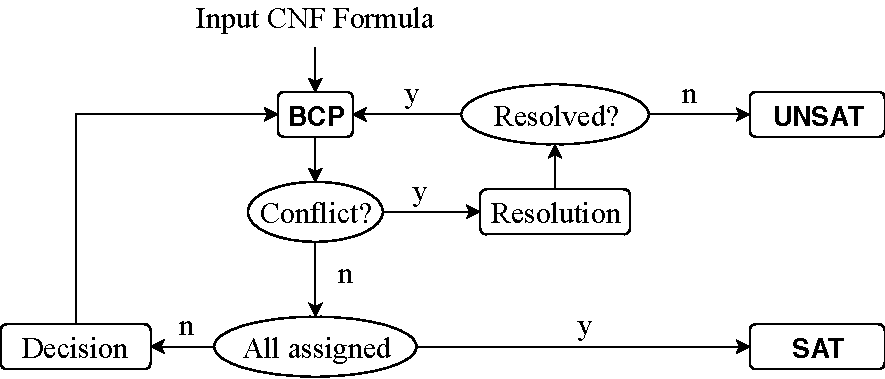
\includegraphics{Images/SAT.pdf}
    \caption{The CDCL framework.}
    \label{fig:cdcl-frame}
\end{figure}
SAT solving aims to check the satisfiability of a propositional logic formula $\varphi$ represented as Boolean combinations of atomic (Boolean) propositions. We introduce CDCL-style SAT solving algorithm, being the most commonly implemented in state-of-the-art SAT solvers.
The CDCL algorithm starts from a CNF formula and then explores the search space by iteratively assigning truth values to some propositions which are chosen according to some heuristic. After each of these assignment the algorithm applies Boolean Constraint Propagation (BPC) to determine the variable assignments implied by the last decision. If the application of BPC leads to a conflict, which is, if the value of a variable is implied to be both true and false at the same time, then \textit{conflict-driven clause-learning} and \textit{non-chronological backtracking} are employed: the algorithm follows back the chain of implication and applies resolution to infer a reason for the conflict in the form of a conflict clause, which then is added to the clause set of the solver. Backtracking removes previous decisions and their implications until the conflict clause can be satisfied. If the starting CNF formula has clauses consisting of a single literal, the algorithm assign them directly. As consequence the algorithm starts with BCP in order to detect implication. If the application of BCP brings to a conflict, the algorithm tries to resolve such conflict. If the conflict is unsolvable then the CNF formula is unsatisfiable, otherwise the algorithm backtracks and continues with BCP. If BCP is completed without conflicts and there are still unassigned propositions, the algorithm makes a new decision. Otherwise the CNF formula is satisfiable and a solution is found.
%
\subsection{Satisfiability Modulo Theories (SMT)}
\begin{figure}[ht]
    \centering
    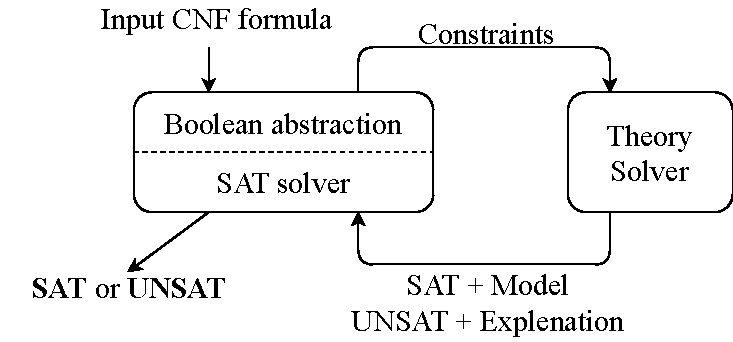
\includegraphics{Images/SMT.pdf}
    \caption{The SMT solving framework.}
    \label{fig:smt-frame}
\end{figure}
Satisfiability Modulo Theories is the problem of deciding the satisfiability of a first-order formula with respect to some decidable theory $\mathcal{T}$. In particular, SMT generalizes the boolean satisfiability problem (SAT) by adding background theories such as the theory of real numbers, the theory of integers, and the theories of data structures (\textit{e.g.}, lists, arrays and bit vectors). To decide the satisfiability of a CNF formulas $\varphi$, SMT solvers usually build a boolean abstraction $\textit{abs}(\varphi)$ by replacing each constraint by a new boolean proposition.
\begin{eqnarray*}
\arraycolsep=2pt
\begin{array}{ccccccccccc}
\varphi &: &\underbrace{x \geq y} &\wedge &(&\underbrace{x > 2}& \vee &\underbrace{y >0}&)& \wedge &\underbrace{y \leq 0} \\
\textit{abs}(\varphi)&:&A& \wedge& (&B& \vee &C&)& \wedge  &\neg C
\end{array}
\label{eq:abs}
\end{eqnarray*}
In the example above $x$ and $y$ are real-valued variable whereas $A$, $B$ and $C$ are boolean proposition.
Once the boolean abstraction is built a SAT solver search for a satisfying assignment $\mu$ for $\textit{abs}(\varphi)$ (e.g. $\mu(A) = \bot$, $\mu(B) = \top$, $\mu(C) = \bot$), if there is no satisfying assignment the CNF formula is unsatisfiable. Otherwise the SMT solver needs to check if the assignment is consistent also in the underlying theory using a \textit{theory solver}. If the theory solver comfirm the consistency of the assignment then a satisfying solution (\textit{model}) is found for $\varphi$. Otherwise the theory solver provides a set of falsified clauses $\phi_T$ which gives an explenation for the conflict, such set is then used to refine the boolean abstraction $\textit{abs}(\varphi)$ to $\textit{abs}(\varphi)\wedge \textit{abs}(\phi_T)$. These steps are iteratively executed until either a theory-consistent Boolean assignment is found, or no more Boolean satisfying assignments exist.